% tocomputer (new_microarchitecture)
%
%\documentclass[10pt,dvips]{article}
%\documentclass[10pt,twocolumn]{article}
\documentclass[10pt,twocolumn]{IEEEtran}
%\documentclass[10pt]{IEEEtran}
\usepackage[english]{babel}
\usepackage{epsfig}
\usepackage{amssymb}
%\usepackage{rotating}
%\usepackage{fancyheadings}
%\usepackage[T1]{fontenc}
%\usepackage[latin1]{inputenc}
%\usepackage{twocolumn}
%\usepackage{verbatim,moreverb,doublespace}
%\usepackage{rotate,lscape,dcolumn,array,rotating,latexsym}
%
%\input{epsf}
%
% for somebody (I forget now !)
%\textwidth 175mm
%\textheight 225mm
%\topmargin -4.5mm
%
% for somebody else (I also forget now !)
%\textwidth 6.6in
%\textheight 239mm
%\topmargin -15mm
%\leftmargin -2.0in
%
% for IEEE (single-column format)
%\textwidth 6.875in
%\textheight 8.875in
%\topmargin -0.6in
%\oddsidemargin 0mm
%\evensidemargin 0mm
%
% for IEEE (two-column format)
\textwidth 6.5in
\textheight 8.875in
\topmargin -0.4in
\oddsidemargin 0mm
\evensidemargin 0mm
%
%
% turn the following (linespread) on to 1.6 for "double space"
\linespread{1.6}
%
%
% some publishers want no page numbers for f{in}al print
%\pagestyle{empty}
%
%
\newtheorem{trans}{Transaction}
\newtheorem{snarf}{Snarfing Rule}
%
\begin{document}
%
% going to 1mm here recoups some good space ! :-)
\parskip 1mm
%\parskip 2mm
%
%
\title{A Distributed Microarchitecture for Realizing High-ILP}
%
\author{
A. {Khalafi}, D. Morano, D.R. Kaeli\\
Northeastern University\\
{{akhalafi}, dmorano, kaeli}@ece.neu.edu\\
\and
A.K. Uht\\
University of Rhode Island\\
uht@ele.uri.edu
}
%
%
% some publishers do not want a data in the f{in}al print
%\date{}
%
%
\maketitle
%
% uncomment the following for page with no page numbers (for IEEE)
%\thispagestyle{empty}
%
%
\begin{abstract}
Many existing programs, and applications in general, are
very serial in nature and cannot easily be parallelized
for gaining execution speed-ups.
Existing conventional microarchitectures have not
been able to extract large amounts of instruction level parallelism (ILP)
from these sorts of programs.
Several problems associated with large ILP
extraction have hindered existing machines from realizing high
instructions per clock (IPC) 
gains on sequential programs.
A primary problem is that the instruction window sizes is not
large enough to bridge control and data dependencies in order
to speculatively execute far enough ahead in the instruction stream.
A larger and more aggressive out-of-order microarchitecture
is needed for this task.
We introduce a new microarchitecture suitable for extracting
large amounts of 
IPC from sequential oriented programs.
Instructions per clocks
in the range of 3.8 to 5.1 are obtained for the
range of machine configurations studied running SpecInt-2000 and
SpecInt-95 programs.
\end{abstract}
%
%
%\vspace{-0.25in}
\section{Introduction}
%\vspace{-0.15in}
%
\PARstart{W}{e} introduce a new distributed microarchitecture for achieving
a high amount of instructions per clock (IPC) from general
sequential program codes.
Lam et al ~\cite{Lam92} showed that a large amount of instruction
level parallelism (ILP) is present within typical program codes.
Results by Uht et al ~\cite{Uht95} confirmed this and showed in more detail
how minimal control dependencies and multipath execution are
important in exploiting ILP.
%
Lipasti and Shen \cite{lipasti96exceeding}
as well as Gonzalez et al ~\cite{Gon97,gonzalez98limits}
showed the potential for ILP through the use of value prediction
in the microarchitecture.
%
Suitable microarchitectures for extracting high ILP would need to
execute a very large number of instructions in parallel.
Unfortunately, conventional microarchitectures currently suffer
from hardware resource contention and routing congestion problems when
scaled to large sizes ~\cite{Palacharla97}.
Particularly severe contention occurs for
microarchitectures using
issue windows,
register update units, or reorder buffers~\cite{Smith95,Bannon95,Kessler98}.
Microarchitectures that have been proposed to attempt to mitigate
the problems associated with large numbers of parallel execution
resources have either relied on assistance from the
compiler, thus rendering them unsuitable for legacy instruction
set architectures (ISA).
Microarchitectures such as the Multiscalar
processor ~\cite{Sohi95} and the Grid Processor Architecture ~\cite{Nag01}
have been of this type.

Many microarchitectural ideas appear to offer potential for
exploiting ILP beyond that of conventional designs.
Some of these ideas include multipath execution,
aggressive control-flow speculation, value prediction, and
memory handling through aggressive memory disambiguation.
Some microarchitectures capable of multipath
execution include those described by Wang ~\cite{Wang90},
Uht and Sindagi ~\cite{Uht95},
Heil and Smith ~\cite{Heil96},
the PolyPath by Klauser et al ~\cite{Klauser98a},
and a simultaneous multithreading oriented approach by
Wallace et al \cite{Wallace98}.
Microarchitectures that attempt to
execute control-independent instructions
beyond the join of conditional branches (minimal control
dependencies) are described by
Sankaranarayana and Skadron ~\cite{Sank01a,Sank01b},
Cher and Vijaykumar ~\cite{Cher01}, and Uht et al ~\cite{Uht01}.
Employing
value speculation ~\cite{lipasti97performance,lipasti98exploiting}
also appears to be a significant advance in exploiting inherent ILP
by breaking the data dependence graph of the program.
A representative microarchitecture of this sort would
be the Superspeculative machine of
Lipasti et al ~\cite{lipasti97superspeculative}.
Aggressive memory handling for large microarchitectures
was also proposed by Franklin et al ~\cite{Franklin96}.
And a promising mechanism for managing the problem of program
execution result ordering was employed in the
Warp Engine ~\cite{Cleary95}.

Our goal was to attempt to combine the best features of
existing microarchitectures and microarchitectural proposals
along with new ways to handle problems associated with existing
designs.
We drew from many of the above ideas and propose a
space-distributed, hardware scalable, grid-oriented microarchitecture
that features: multipath execution, minimal control
dependencies, value prediction, aggressive memory speculation and
handling, and time tags for maintaining program dependency order.

The rest of this paper is organized
as follows.
Section~\ref{sec:rfem} introduces a new model for guiding program execution
and the management of machine hardware resources during execution.
This new execution model is termed \emph{Resource Flow Execution}.
Section~\ref{sec:rfma} provides the description of a microarchitecture
that realizes our Resource Flow execution model.
Section~\ref{sec:eval} provides an experimental evaluation of 
the effectiveness of the described microarchitecture.
%
%
%
\section{Resource-Flow execution model}
\label{sec:rfem}
%
To take advantage of the large amounts of instruction level
parallelism available in current sequential programs it is
necessary to speculate beyond the traditional control and data flow
dependency constraints and allow for more
parallel execution of the code (albeit speculative).  
In current microarchitectures that
perform speculative execution, access to the reorder buffer becomes
very problematic as the number of instructions being speculatively
executed concurrently grows~\cite{Palacharla97}.
This is mainly due to the
contention for the centralized resources, such as data registers, within
the reorder buffer.
We are proposing a new microarchitecture that exploits highly speculative
execution through a \emph{Resource Flow} execution model to achieve high
levels of IPC.  
In the Resource Flow execution model instructions
with the highest priority are
assigned to free execution resources regardless
of whether the input operands of the instructions have the f{in}al correct
value (data flow constraints) and regardless of the outcome of the
previous branches in the instruction stream (control flow constraints).
This means that the execution is guided
only based upon the need for an instruction to execute and
the availability of resources.  The rest of the execution
time is spent re-executing the instructions that have had an incorrect
speculative input or operand, so as to end up with a programmatically
correct execution of the code.  As demonstrated in the rest of this
section, the Resource-Flow execution model does not require
explicit renaming of registers or any reorder buffers, which accordingly
would eliminate the contention for centralized resources.
This model provides methods for executing standard procedural (control-flow
guided) programs
that go beyond the standard control and data flow model.

\subsection{Time Tags}

In the Resource-Flow execution model, instructions are executed
speculatively in an out-of-order fashion.  We use time-tags to enforce
the correct data and control dependencies among the instructions to
realize speculative data-flow execution of code.  A time-tag is a small
integer that uniquely identifies the position of an instruction or an
operand in program ordered time with respect to the most recently
retired instructions.
%
%Time-tags are used in common processors to
%squash instruction results occurring after a mispredicted branch, as
%well as to maintain instruction order in general [].
%
The application of time-tags to keep track of the original instruction 
order, as is used in our microarchitecture, was originally 
proposed in the Warp Engine~\cite{Cleary95}.
This machine, however, had to use floating point numbers
for time-tags since they needed to create an arbitrary number of time-tags
between any given pair of time-tag.  
In our microarchitecture, 
time-tag values are associated with
the equivalent of
the issue slots in an instruction window and
take on small integer values.

To assign the time-tags, the oldest issued instruction in flight that
is neither yet committed nor squashed would usually have a time-tag
value of zero.  More recently dispatched instructions take on
increasingly larger values the further ahead they are in the program
ordered instruction stream.  As a group of instructions with the lowest
valued time-tags are retired, all of the time-tags for all instructions
and operands are decremented by the number of instructions just
retired.  
This prevents time-tags from
growing indefinitely.
Therefore the next instruction in program order to be retired will
have the time-tag value of zero.
%
%
\subsection{Operand Transactions}
%
Both renaming and time-tagging assume that results from the execution
of an instruction are put on a bus and snooped by all later
instructions. 
In the resource flow model, the forwarding of the
identifying address of the output operand and its value is
accompanied with the instruction time-tag and
path~ID~\cite{Skadron01} (if multipath execution is allowed).  
The
time-tag and path ID will be used by subsequent instructions in
program order to determine if the operand with the desired
address originated from the closest previous
instruction and therefore should be \emph{snarfed}\footnote{Snarfing 
implies we snoop a bus and if a match on the current bus contents is
found, we read the associated data value.}.
A snarfed
value could subsequently trigger the execution or re-execution of
the instruction.

Communication between instructions is realized through a set of
transactions that we call \emph{Operand Transactions}.  
There are two
general forms of transactions, namely \emph{forward} (FW) and
\emph{backward} (BW) transactions.  
A forward transaction sends
(forwards) information to the instructions later in the program
execution order.  
A backward transaction sends requests to the
earlier instructions in the program execution order.

In order to correctly execute the program instructions and to process 
the operand transactions, each instruction that has been dispatched (to
what conventionally would have been an issue window slot) is extended
by associating a data structure with it.
This
data structure is used to hold the transaction-specific information
as well as intermediate operand values.  
The combination of an
instruction and its associated data structure is termed an
\emph{Active Station} (AS).  
The term active station is derived from the idea that it holds an
instruction for its entire duration of time in-flight.
The set of all active stations along with all of the execution 
resources in the machine is termed the \emph{Execution Window}.
Control-flow and data-flow dependencies are
enforced through communication between active stations using a set
of transactions.  
Active stations constantly examine
transactions that they see. 
If the information in a transaction that has been transmitted by
some AS is
needed for the execution of the instruction in another AS, the
associated data is snarfed by the receiving AS. 
The following list shows the different data 
structures used in an active station $AS_i$, where $i$ is the physical 
index of the active station.
%
\vspace{0.2 in}
\begin{list}{\mbox{}}
\item
\item $\mathbf{AS_i.en}$ is a binary value which is set 
to one if the Instruction is enabled
and its result is used in the execution of the program.
\item $\mathbf{AS_i.tt}$ holds the time-tag value.
\item $\mathbf{AS_i.op_x}$ where $x \in \{1,2,\ldots\}$ holds the 
input operands of
the instruction $I_i$ residing in the active station.
\item $\mathbf{AS_i.op_x.last\_tt}$ holds the source time-tag 
of the last snarfed
transaction that its data was used in the 
execution of the $I_i$ ;
since each operand
can have a different source, a separate variable for each operand is needed
\item $\mathbf{AS_i.D}$ is the address of the output operand of $I_i$.
\item $\mathbf{AS_i.D.data}$ is the value of the $AS_i.D$ operand.
\item $\mathbf{AS_i.mem.addr}$ holds the memory 
address (valid only if $I_i$ is a load or store instruction)
\item $\mathbf{AS_i.mem.data}$ holds the memory 
value (valid only if $I_i$ is a load or store instruction)
\item $\mathbf{AS_i.mem.last\_tt}$ holds the source time-tag 
of the last memory
value that was snarfed (valid only if $I_i$ is a load instruction)
\item $\mathbf{AS_i.D.last\_data}$ holds the output operand value 
produced by the
last enabled instruction before $I_i$ ; in case $I_i$ is disabled, 
this value is
forwarded as the correct value of the destination register
\item $\mathbf{AS_i.outcome}$ is a binary value set according to 
the outcome of the branch
(valid only if $I_i$ is a branch instruction)
\item $\mathbf{AS_i.target\_tt}$ holds the time-tag of the branch 
target instruction
(valid only if $I_i$ is a branch instruction)
\item $\mathbf{AS_i.CEPB}$ structure holds the information 
regarding the \emph{Closest Enabled Previous Branch} (CEPB)
with respect to instruction $I_i$ in
the static program-order ; this is used to handle predicate assignment and 
evaluation
More information will be provided in Section~\ref{sec:hwpred}
\end{list}
%
\vspace{0.2 in}

In following sections we provide examples showing how the
above data structures are used to enforce the correct program execution.
We will introduce a set of transactions that are employed in our Resource
Flow execution model to
communicate data and predicates between different active stations.
%
\begin{figure*}[th]
\centering
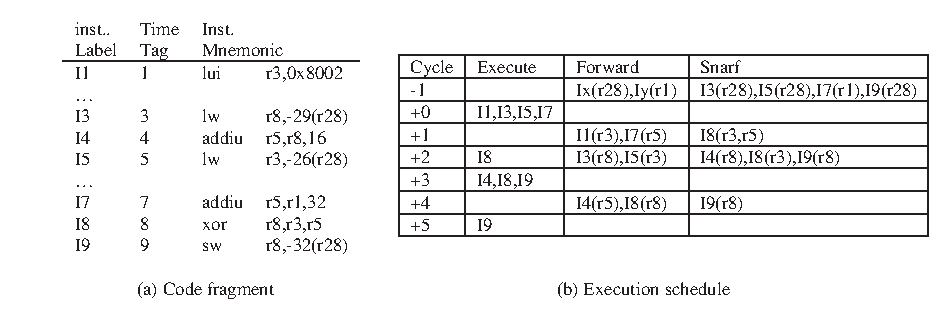
\epsfig{file=ttexec.eps,width=5.0in}
\caption{{\em Example instruction execution.}
Part (a) shows a fragment of a MIPS ISA program, code along with the
time-tags assigned to the instructions.
Part (b) shows the schedule of execution, forwarding, and snarfing
events that facilitate operand acquisition by the instructions.}
\label{fig:ttexample}
\end{figure*}
%
%
\subsection{Register Operation}
\label{sec:regop}
%
In our microarchitecture, instruction operands are of three basic
types.  These are associated with registers, memory locations,
and predicates.  Register and memory operands communicate architected
(defined as part of the ISA) while the predicate transactions
are not architecturally visible but are used within the microarchitecture
itself for program control-flow dependency enforcement.
In our microarchitecture, similar to others,
these operands are treated rather differently. 
In this section we describe
how register operations are handled in our Resource Flow execution model.

We introduce the following transactions and show that they are
adequate for handling register operations in our
microarchitecture :

\begin{trans}
\mbox{} \\
\indent $trans.name \leftarrow RegVal $ \\
\indent $trans.type \leftarrow FW $ \\
\indent $trans.tt \leftarrow AS_i.tt$ \\
\indent $trans.op \leftarrow AS_i.D $ \\
\indent $trans.data \leftarrow AS_i.D.data $
%\flushright{$\diamondsuit$}
%\flushright{$\blacksquare$}
\end{trans}

\begin{trans}
\mbox{} \\
\indent $trans.name \leftarrow Relay$ \\
\indent $trans.type \leftarrow FW$ \\
\indent $trans.tt \leftarrow AS_i.tt$ \\
\indent $trans.op \leftarrow AS_i.D $ \\
\indent $trans.data \leftarrow AS_i.D.last\_data $
\end{trans}

%This transaction forwards the destination register operand of an instructions
%along with its time tag.

%If instruction $I_i$ is disabled, its output
%register operand value is no longer valid.  This transaction
%announces this to the following instructions and sends out the
%previous value of the output operand.

Note that previous values of the instruction output operand are
snooped and the latest value is always stored in
$AS_i.D.last\_data$ register.  
If the instruction predicate
changes from disabled to enabled, the output operand that was
computed by the instruction is forwarded.  If the instruction
predicate changes form enabled to disabled, the previous value of
the output operand (before being changed due to the instruction
execution) is forwarded.  With this strategy, instructions that
are located in the program-ordered future will eventually
get the correct value that will end up being the committed value
if the current instruction ends up being committed itself.  This
is a simple and effective forwarding strategy, which makes it a
reasonable choice for handling register operations.  The inclusion
of the time tag in the transaction is the key element that allows
for the correct ordering of dependencies in the committed program.

Another task of an active station is to snoop for new operand values
and snarf them if necessary.
%
%Figure~\ref{fig:source} shows the
%detailed snooping hardware for an input operand of an Active
%Station. As can be seen,
%
A new operand is snarfed when it has the
same address as an operand in the current active
station and it is from a previous (in program ordered time) active station
whose program-ordering is 
equal or greater than that of the source of the previously held operand.
Further, if the current active station did not have any value for the operand
being snooped, it will snarf any operand from any previous (in 
program-ordered time) active station that produces one.
Snarfing rule~\ref{snar:regop} summarizes the above statement.
As the description of the snarfing rule shows, the time-tag 
value of the snooped operand
is compared with the time-tag of the current active station 
and the time-tag of the last snarfed operand.  
If the newly arrived 
operand is later in program order time than the previously snooped
operand, it will substitute the previously held value.

\begin{snarf}
\label{snar:regop}
\mbox{} \\
\(
\begin{array}{ll}
(trans.name = RegVal\ & \textup{or} \\ trans.name = Relay) & \textup{and} \\
AS_i.op_x.last\_tt \leq trans.tt < AS_i.tt  & \textup{and} \\
AS_i.op_x.addr = trans.op.addr \\
\hspace{3em} \Rightarrow \\
AS_i.op_x.last\_tt \leftarrow trans.tt\\
AS_i.op_x.data \leftarrow trans.data
\end{array}
\)
\end{snarf}

A similar snarfing rule deals with the output operand values.

\begin{snarf}
\label{snar:outregop}
\mbox{} \\
\(
\begin{array}{ll}
(trans.name = RegVal\ & \textup{or} \\ trans.name = Relay) & \textup{and} \\
AS_i.D.last\_tt \leq trans.tt < AS_i.tt & \textup{and}\\
AS_i.D.addr = trans.op.addr \\
\hspace{3em} \Rightarrow \\
AS_i.D.last\_tt \leftarrow trans.tt\\
AS_i.D.last\_data \leftarrow trans.data
\end{array}
\)
\end{snarf}

Figure ~\ref{fig:ttexample} is an example of how the Resource Flow
model is used to enforce correct execution of instructions by
enforcing data dependencies.  Part (a) shows a fragment of a MIPS ISA
program code. 
Each instruction is assigned to an active station with a
unique time-tag value.  
Figure~\ref{fig:ttexample}.b illustrates the
steps required to execute this code fragment. 
For simplicity, in
this example we assume that there are no branches among these
instructions and that they are all predicted to be executed.
It is also assumed
that there is no constraint on the number of execution units available and
that the number of transactions that can be forwarded in each cycle is
infinite.
The f{ir}st column shows the clock cycle times.  The next
three columns list the instructions that are either executing,
forwarding an operand, or snarfing a snooped operand value.  The
notation that is used is $I_x(r_y)$ where $I_x$ is the instruction
label and $r_y$ is the register that is either forwarded or
snarfed.  Note that snarfing is done in parallel with instruction
execution and transaction forwarding.

At cycle +0, instructions $I_1$, $I_3$, $I_5$ and $I_7$ are
executed in parallel.  The execution is the result of the snarfing
of new values for the $r1$ and $r28$ registers in the previous cycle.
Assuming two cycles for the execution of load and store
instructions, and one cycle for the rest of the instructions in
this example, instructions $I_1$ and $I_7$ will produce their
results in the next clock. 
The new value for registers $r3$ and
$r5$ are forwarded in cycle +1 and are snarfed by instruction
$I_8$. 
In the next cycle, instruction $I_8$ will be executed using
its newly read register value.  Normally $I_8$ should forward the
new result, but since $I_5$ is sending out a new value for $r3$,
the $I_8$ instruction snarfs the new value of $r3$.  This results
in re-execution of the $I_8$ instruction in cycle +3.  In the next
cycle, $I_4$ sends a new value for register $r5$ with a time-tag
of 4, but since the last value of $r5$ received by $I_8$ had a
time-tag of 7, which is greater than 4, the new value is ignored
by $I_8$ and does not result in another re-execution.
%
%
\subsection {Hardware Predication}
\label{sec:hwpred}
%
Predicated execution is shown to be an effective approach for
handling conditional branches~\cite{Mahlke92}. 
In our microarchitecture, the
predicates are generated at run-time.  Each instruction computes
its own enabling predicate by snooping for and snarfing predicate
operands that are forwarded to it by earlier instructions from the
program-ordered past.  They are evaluated solely with hardware,
and are not architecturally visible thus allowing for the use of 
the method with legacy ISAs and program codes.
Full hardware based predication
is a new way to manage and achieve minimal control dependencies
(MCD).  With MCD, all branches may execute concurrently and the
instructions after a \emph{branch domain} ~\cite{Uht91} may execute
independently of the branch.  A branch domain is defined as the 
set of instructions
that fall between the branch and its target instruction.
%
\begin{figure}
%\vspace{0.2 in}
%\setlength{\epsfxsize}{10cm}%7
%\centerline{\epsfbox{window.eps}}
%\centering
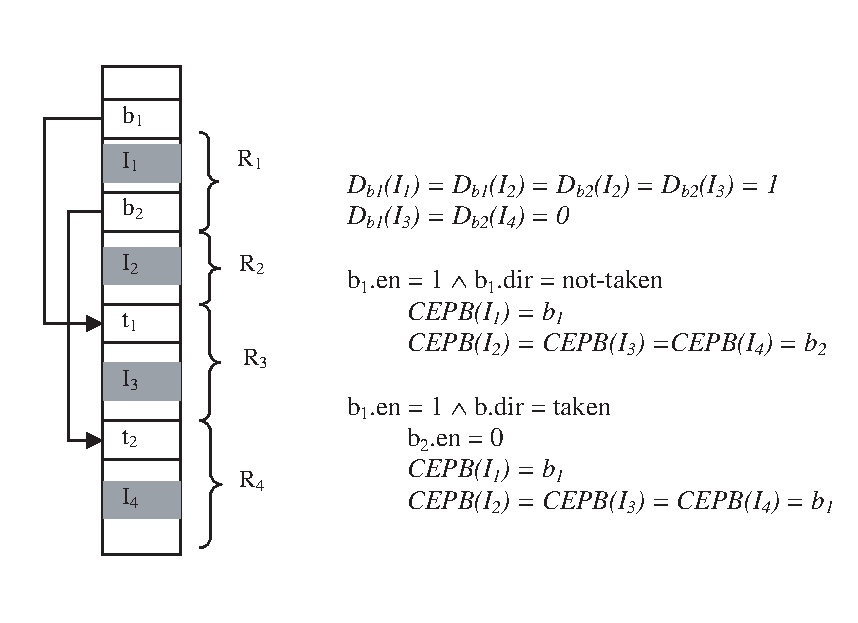
\epsfig{file=brdomain.eps,width=3.0in} 
\caption{{\em Branch Domain and Closest Enabled Previous Branch.} 
A representation of an instruction sequence in
static program (memory) order is shown along with the regions
that are created by the presence of conditional branches.}
\label{fig:brdomain}
\end{figure}
%
We propose a hardware predication mechanism that
can be implemented using our resource flow methodology. 
This scheme allows branches to execute concurrently and 
in an out-of-order fashion
while also guaranteeing that all instructions will get their 
correct predicate value.
Figure~\ref{fig:brdomain} shows a program code sequence with two
branches $b_1$ and $b_2$  and their corresponding targets $t_1$ and
$t_2$.  The two branches divide the code into 4 regions.  The
execution of the instructions in regions $R_1$, $R_2$ and $R_3$
depends on the outcome of branches $b_1$ and $b_2$, whereas the
instructions in $R_4$ are executed independent of the branch
outcomes.  A scheme is used for
assigning an enabling predicate to every instruction in each
region based on the outcome of branches.  If the enabling
predicate value is one, then the instruction will be executed;
otherwise it is disabled.  The following definitions are used in
the description of our scheme.

\begin{description}[\setlabelwidth{CEPB(Ij)xxx}]
\item[$T(b)$:] a binary value, set to one if the branch $b$ is
predicted taken
\item[$en(I_j)$:] a binary value assigned to each
instruction $I_j$ which specifies whether the instruction is
enabled for execution.
\item[$D_b(I_j)$:] a binary value,
set to one if the instructions $I_j$ is in the domain of branch $b$.
\item[$CEPB(I_j)$:] Closest Enabled Previous Branch to instruction
$I_j$ in the static program-order.
\end{description}

In Figure ~\ref{fig:brdomain} we have also shown 
the value of the $CEPB$ and $D_b$ variables for the
two branches in the f{ig}ure.
The $D_b(I)$ function is
independent of the outcome of the branch and only depends on the
static order of the instructions in the code.  $CEPB(I)$, on the other
hand, is a function of the outcome of other branches and will
change during the course of speculative execution.

Using the above definitions, we can show that:
%
\begin{equation}
\overline{en(I_j)} = T(b) \cdot D_b(I_j)  \textstyle{\ where\ } b = CEPB(I_j)
\label{eq:preden}
\end{equation}
%
\textsc{Proof:} The proof is through induction.  Assume
$b_1$, $b_2$, $\cdots$, $b_n$ are $n$ earlier branches before
instruction $I_j$.
If $n = 1$ then $CEPB(I_j) = b_1$.  $I_j$ is disabled if and only if it is
in the domain of $b_1$ and $b_1$ is a taken branch.  In other words
$\overline{en(I_j)} = T(b_1) \cdot D_{b_1}(I_j)$ which is the 
same equation as~(\ref{eq:preden}).

Now let's assume that equation~(\ref{eq:preden}) is valid when there are
$n$ branches before $I_j$.  We show that
equation~(\ref{eq:preden}) is also valid when there are $n+1$ branches before
instruction $I_j$.
Since there are only $n$ branches before $b_{n+1}$, we can write:
%
\begin{equation}
\overline{en(b_{n+1})} = T(b_x) \cdot D_{b_x}(b_{n+1}) \\
\label{eq:pr12}
\end{equation}
%
where \ $b_x = CEPB(b_{n+1})$.
Also from the definition of CEPB, we have:
%
\begin{equation}
CEPB(I_j) = \left\{ \begin{array}{ll}
    b_{n+1} & \mbox{if $en(b_{n+1}) = 1$} \\
    CEPB(b_{n+1}) & \mbox{}
    \end{array}
    \right.
\label{eq:pr11}
\end{equation}
%
If $en(b_{n+1}) = 0$ then branch $b_{n+1}$ will not have 
any effect on the execution of $I_j$.  
From~(\ref{eq:pr11}) we
can see that \mbox{$b_x = CEPB(I_j) = CEPB(b_{n+1})$}.  
Since $b_x$ is 
within one of the last $n$ branches before $I_j$ from
the assumption 
\mbox{$\overline{en(I_j)} = T(b_x) \cdot D_{b_x}(I_j)$} which is 
the same as equation~(\ref{eq:preden}).

Next we consider the case where \mbox{$en(b_{n+1}) = 1$}.
Since there are no other branches between $b_{n+1}$ and $I_j$, instruction
$I_j$ is enabled unless it is in the domain of $b_{n+1}$ and $b_{n+1}$ is
a taken branch.  In other words:\\
\mbox{$\overline{en(I_j)} = T(b_{n+1}) \cdot D_{b_{n+1}}(I_j)$}.
But since \mbox{$en(b_{n+1}) = 1$}, 
from~(\ref{eq:pr11}) we see that \mbox{$CEPB(I_j) = CEPB(b_{n+1})$}
and therefore equation~(\ref{eq:preden}) is valid.

Equation~(\ref{eq:preden}) simply tells us that if instruction $I_j$ is in
the domain of an enabled branch, and if the branch is taken, $I_j$ will
not be executed.  If the instruction is out of the domain of its closet
enabled previous branch, then its execution is independent of the
outcome of the branch.

Equation~(\ref{eq:preden}) is the basis for our dynamic predication scheme.
The following two transactions, along with the snarfing rule, are used
to implement a mechanism for dynamic assignment of predicates 
to each instruction.

\begin{trans}
\mbox{} \\
\indent $trans.name \leftarrow PredVal $ \\
\indent $trans.type \leftarrow FW $ \\
\indent $trans.tt \leftarrow AS_i.tt$ \\
\indent $trans.dir \leftarrow AS_i.outcome $ \\
\indent $trans.target \leftarrow AS_i.target $
\end{trans}

\begin{trans}
 \mbox{} \\
 \indent $trans.name \leftarrow PredInv$ \\
 \indent $trans.type \leftarrow FW $ \\
 \indent $trans.tt \leftarrow AS_i.tt$ \\
 \indent $trans.new\_tt \leftarrow AS.CEPB.tt $ \\
 \indent $trans.dir \leftarrow AS_i.CEPB.outcome $ \\
 \indent $trans.target \leftarrow AS_i.CEPB.target $
\end{trans}

\begin{snarf}
\label{snar:predval}
\mbox{} \\
\(
\begin{array}{ll}
(trans.name = PredVal \ & \textup{or} \\ trans.name = PredInv) & \textup{and} \\
AS_i.CEPB.tt \leq trans.tt < AS_i.tt \\
\hspace{3em} \Rightarrow \\
AS_i.CEPB.tt \leftarrow trans.tt\\
AS_i.CEPB.outcome \leftarrow trans.outcome\\
AS_i.CEPB.target \leftarrow trans.target
\end{array}
\)
\end{snarf}

To assign the predicate value to each instruction $I_j$, it is sufficient
to find the $CEPB(I_j)$ branch and its outcome.  This is a simple
task in our scheme.  Each active station has a pair of $AS.CEPB.tt$
registers to hold the time-tag of its current $CEPB$ branch and
corresponding target.  If an earlier branch is enabled, a
\emph{PredVal} transaction is sent on the forwarding bus with
the time-tag of the branch, its target address, and whether it is a taken
branch or not.  Each subsequent active station, such as $AS_i$,
that snoops this
transaction checks to see if the time-tag of the newly enabled
branch is greater than its current $AS_i.CEPB.tt$ value. 
If it is, the new
branch is closer to this instruction and therefore it will replace
the older $CEPB$ branch.

If a branch such as $b$ becomes disabled, the later instructions need
to find another branch as their new $CEPB$ branch.  This new branch 
is simply $CEPB(b)$, because according to the definition there is 
no other enabled
branch between $CEPB(b)$ and $b$. 
In
our scheme this is achieved by initiating a \emph{PredInv} transaction
at branch $b$.  An invalidate transaction contains the time-tag of
$b$, the time-tag of $CEPB(b)$, and the branch domain information of
$CEPB(b)$.  This information was snooped by $b$ when $CEPB(b)$
forwarded its output predicate.

To find the domain of a $CEPB$ branch, a simple approach is to just
compare the branch target address with the instruction address.
It is however more efficient to use time-tags for this purpose.
A branch really only needs to forward the time-tag of its target
instruction instead of its target address.  The branch target
time-tag can be easily calculated by adding the branch
displacement to the branch time-tag value.

Another improvement to the above scheme can be made by observing
that a not-taken enabled branch does not need to send out any
transaction on the forwarding bus.  This is due to the fact that a
not taken branch essentially acts like a NOP operation.  The
advantage is a reduction of the number of transactions on the 
communication bus.
%
\begin{figure}
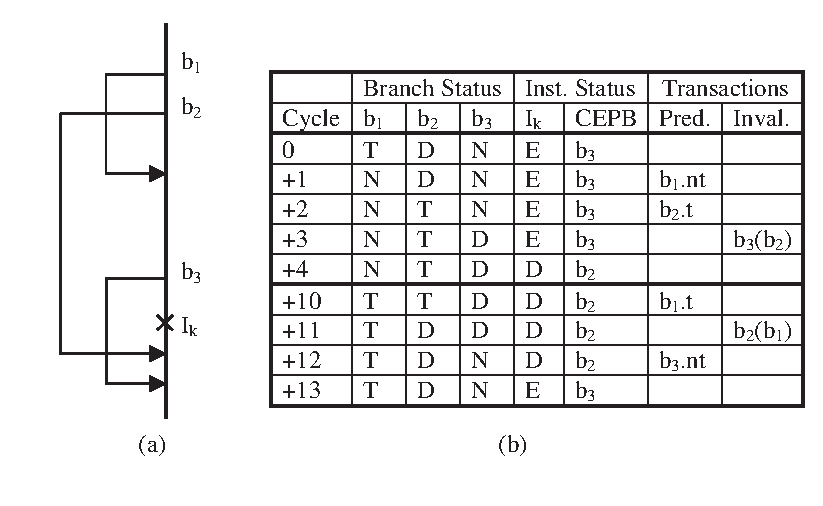
\epsfig{file=dynpred.eps,width=3.0in} 
\caption{{\em Example Illustrating Dynamic Predication.}
Part (a) shows the flow of instructions in static program (memory) order
along with the control flow outcomes of a number of conditional branch 
instructions.  Part (b) show the timing and events of execution
that facilitate dynamic control-flow predication of the code sequence.}
\label{fig:dynpred}
\end{figure}
%
Figure~\ref{fig:dynpred} shows an example of how our dynamic
predication work.  The f{ir}st column in the table lists the relative
clock cycles.  The next three columns list the status of each
branch.  The "D", "T' and "NT" entries correspond to disabled,
taken and not-taken status, respectively.  The next two columns
list the $I_k$ instruction status.  The entry designations "E" and "D" 
stand for enabled
and disabled status, respectively.  The column labeled $CEPB$ shows the
$CEPB(I_k)$ branch at any cycle.  The next two columns show the
transactions on the bus.  The "PredVal" column lists the predicate
forwarding transactions for each branch along with its status.  The
"PredInv" column lists the invalidating transactions.  The branch
name in the parenthesis corresponds to the new $CEPB$ forwarded by
the invalidated branch.

In the example it is assumed that branches $b_1$ and $b_3$ are initially
predicted taken and not-taken, respectively.  
As a result instruction $I_k$ is predicated enabled.  
In the next cycle, $b_1$ changes its direction to a
not-taken branch and sends a forwarding transaction on the bus.
This transaction will enable branch $b_2$, which is also predicted taken.
Branch $b_2$ will send a predication transaction on the forwarding bus
that is snooped by branch $b_3$.  
As a result, branch $b_3$ will be disabled in
cycle 3 and will send an invalidating transaction with $b_2$ as
its $CEPB$ branch.  Instruction $I_k$ will see this transaction and
switch its $CEPB$ to $b_2$, and will also be disabled.  
The
second part of the table (part b) in Figure ~\ref{fig:dynpred} 
(clock cycles 10 through 13 inclusive) shows what
will happen if $b_1$ changes back to a taken status.  
A new set of transactions will follow that will eventually enable 
instruction $I_k$.

In the previous example we saw that $I_k$ was f{ir}st disabled and
then enabled.  
A disabled instruction needs to notify later
(later in dynamic program order)
instructions that its destination register value, which could have
been forwarded earlier, is no longer valid (it has changed).  
Further, any disabled instruction has to
send the previous (previous to it) destination value from 
the closest enabled previous
instruction as the correct value.  
In section~\ref{sec:regop} we showed that 
a \emph{Relay}
transaction can be used to send out the previous value as the current
correct value.
The disabled instruction, in effect,
acts like a relay and will forward the earlier value using its own
time-tag.  
Note that it is important that the disabled instruction forward
the previous operand value with its own time-tag value since
any subsequent snooping instructions will ignore all operand
transactions (with the designated operand address) with time-tag
values lower than that of the disabled instruction.
A disabled memory store operation, on the other hand, 
need to invalidate its output value.  In the next section, we will explain
why this is need and how this is done through a \emph{nullify} transaction.

As demonstrated by this example, the cost of hardware predication
is low and most of the extra state only uses a few
bits of storage in the active station component.  
This hardware s the same for all active stations in the machine.
%
%
\subsection {Memory Operations}
%
With the increasing number of instructions in flight, there is 
increasing probability
that the memory values generated by store operations will
be used by load operations that are also in-flight in the machine
at roughly the same time.  
Our measurements, shown and discussed 
in section~\ref{sec:segbus},
show that over 30\% of all load operations can obtain their operand values
directly from a store operations that preceded it
without having
to go to a higher level in the memory hierarchy.  
Satisfying load requests without resorting to higher levels of the
memory hierarchy (like the L1 data cache) should relieve contention
pressure on the L1 data cache (and other memory levels) and
improve overall machine performance.

To enforce the true memory dependencies, we use a similar
forwarding and snooping mechanism introduced in
section~\ref{sec:regop}.  However, we cannot use the same
\emph{RegVal} transaction as was done with register operands.  
Unlike register operands which have
a fixed architected address for any single instruction operand, the
address of a memory operand for an instruction is not necessarily fixed.  
This is because of the use of register indirect addressing for memory
variables in most architectures.
The memory
address is often computed using a the sum of a fixed displacement and a
register value in many ISAs.  
Since the value of most all register operands in the machine are
speculative, any derived memory addresses from those register
operands are also speculative.
For store instructions, if the address of the memory store
changes, the instruction has to have a way to notify later
instructions (in dynamic program order) that any previously 
transmitted memory operand values for that address may be 
(and most likely are) invalid.  
This contrasts with the register operand case since in that case a previous
value of the register can simply be transmitted to correct any
wrong values that were transmitted.
However, in the case of memory operand, the previous value of a
memory location is not known (since that would have required the
equivalent of a load request itself to have acquired that value)
so instead the value that was transmitted previously by the current
store instruction needs to invalidated in some way.
Because of this differences between register operand handling
and that of memory operands, the following
transaction is used for forwarding memory values to
later load instruction :
%
\begin{trans}
 \mbox{} \\
 \indent $trans.name \leftarrow MemVal$ \\
 \indent $trans.type \leftarrow FW$ \\
 \indent $trans.tt \leftarrow AS_i.tt$ \\
 \indent $trans.mem.addr \leftarrow AS_i.mem.addr $ \\
 \indent $trans.mem.data \leftarrow AS_i.mem.data $
 \end{trans}
%
The associated snarfing rule is:
%
\begin{snarf}
\label{snar:memval}
\mbox{} \\
\(
\begin{array}{ll}
trans.name = MemVal & \textup{and} \\
AS_i.mem.last\_tt \leq trans.tt < AS_i.tt & \textup{and}\\
AS_i.mem.addr = trans.mem.addr \\
\hspace{3em} \Rightarrow \\
AS_i.mem.last\_tt \leftarrow trans.tt\\
AS_i.mem.data \leftarrow trans.data
\end{array}
\)
\end{snarf}
%

There are, however, limitations to the
usefulness of the above transaction.  The speculative nature of
this microarchitecture could result in temporary incorrect
register values for the memory operations.  As a result, the load or
store memory address could be wrong.  A load operation that snoops
for an incorrect memory address will miss the opportunity to snarf
the correct memory value forwarded by a previous store operation.
It is therefore necessary for a load operation to eventually
initiate a memory request using its resolved memory address.  In
traditional microarchitectures, the request normally goes to the
f{ir}st level D-cache.  In our proposed microarchitecture, there is
a good chance that the correct memory value is still in the
execution window and has not yet been written back to the higher
level memory.  Based on this observation, we send memory requests
to both higher level memory and previous active stations.  If
there is any store operation with the same address in earlier
active stations, it will forward the memory value, which will
subsequently snarfed by the load instruction.  Otherwise the
memory value received from the higher level memory is used.

The requests to previous active stations Stations are handled using the
following backwarding (backward going) transaction.  
This transaction is similar to
the \emph{MemVal} transaction introduced above except that 
it is primarily used to
send data requests to the instructions earlier in the program
order.
%
\begin{trans}
\mbox{} \\
\indent $trans.name \leftarrow MemReq$ \\
\indent $trans.type \leftarrow BW$ \\
\indent $trans.tt \leftarrow AS_i.tt$ \\
\indent $trans.mem.addr \leftarrow AS_i.mem.addr $
\end{trans}
%
The only data that are sent in this transaction is the 
time-tag of the active station
and the memory address.  The closest previous store operation with the same
memory address will forward its value upon receiving the above
transaction.

Another difficulty with the application of the forwarding and
snooping strategy for memory operations (as mentioned previously)
is that a store operation
with an incorrect memory address could forward an erroneous value
that will be incorrectly snarfed by another load operation with
the same address.  This seems to present a problem for the correct
enforcement of memory operand dependencies but 
the solution is straightforward.

The load instruction that snooped the f{ir}st MemVal transaction from the store
instruction has kept a copy of the store instruction's 
time-tag in $AS.mem.last\_tt$
register.  When the load snoops the second MemVal transaction from the store
it notices the difference between its memory address and $trans.mem.addr$
forwarded by the store instruction.  This means that the store has changed
its address and the load needs to initiate a MemReq transaction.
However, there is still a need for another type of transaction.  A store
instruction that receives a disabling predicate needs to notify the subsequent
load instructions to ignore any value that was previously forwarded by 
that store instruction.  We define \emph{MemNul} transaction as 
a new type of operand transaction with the property of
\emph{nullifying} the effect of a previous store transaction.
%
\begin{trans}
\mbox{} \\
\indent $trans.name \leftarrow MemNul$ \\
\indent $trans.tt \leftarrow AS_i.tt$ \\
\end{trans}
%
This transaction is seen by all
later load instructions.  Any load instruction that has snarfed a
value sent from that specific store instruction will ignore the
value and will initiate a new request to the memory using a \emph{MemReq}
transaction.
%
%
\subsection{Summary}
%
Table~\ref{tab:asop} summarizes the operations carried out by an
active station based on the type of the issued instruction and the
snarfed values.  The f{ir}st column in this table shows the instruction
type.  The second column shows the snarfed data.  
The content of these two columns
determines the operation carried out by the active station as is
shown in third column.  The last two columns list the transactions
that will be initiated by the active station based on the value of
the enabling predicate of the instruction in the active station.

As an example, if an enabled load instruction receives a value for its
output operand $r$, it will save its value in AS.D.last\_data (last\_r in
the table).  If at some time in the future this same load instruction receives a disabling
predicate, it will initiate a Relay transaction and send out the last value of
register $r$ as its correct value.

\begin{table}
\begin{center}
\caption{active station Operation} \label{tab:asop} \scriptsize{
\begin{tabular}{|l|l||l|l|l|}

\hline Instruction & Snarfed & AS &
\multicolumn{2}{c|}{Transaction}\\ \cline{4-5}
Type & Data & Operation & enabled AS & disabled AS \\
\hline

 & a or b & execute & RegVal & - \\
 \emph{Register} & c & last\_c $\leftarrow$ c & - & -\\
 c $\leftarrow$ a \emph{op} b & en\_pred & - & - & RegVal \\
 & dis\_pred & - & Relay & - \\

 \hline

 & a & calc addr & MemReq & - \\
 \emph{Load} & M[a] & - & ReqVal & - \\
 r $\leftarrow$ M[a] & r & last\_r $\leftarrow$ r & - & -\\
 & en\_pred & - & - & RegVal \\
 & dis\_pred & - & Relay & - \\

 \hline

 & a & calc addr & MemNul & - \\
 \emph{Store} & r & - & MemVal & - \\
 M[a] $\leftarrow$ r & en\_pred & - & - & MemVal \\
 & dis\_pred & - & MemNul & - \\

 \hline

 & a or b & compare & PredVal & - \\
 \emph{Branch} & en\_pred & compare & - & PredVal \\
 br a,b,target & dis\_pred & - & PredInv & - \\

\hline

\end{tabular}
}
\end{center}
\end{table}
%

%
%
\section {A Resource Flow Microarchitecture}
\label{sec:rfma}
%
In this section we present an ISA independent, distributed
microarchitecture that uses the Resource Flow execution model and some of
the most desirable features of proposed future microarchitectures in order to
achieve higher IPC.  
Desirable microarchitectural features are 
control flow speculation, data value speculation,
execution of control-flow independent instructions, and multipath execution.  
We attempt to employ all of these features in the present microarchitecture.
The microarchitecture is
very aggressive in terms of the amount of speculative execution it
performs.  
This is realized with a large amount of 
execution resources.  
Hardware scalability of the microarchitecture is
achieved through its distributed nature along with repeater-like
components that limit the maximum bus spans.  
Contention for major
centralized structures such as register file, reorder buffer, and
centralized execution units is eliminated through distribution of
theses resources.

A high level diagram of our microarchitecture is shown in
Figure ~\ref{fig:highlevel}.  
%
\begin{figure}
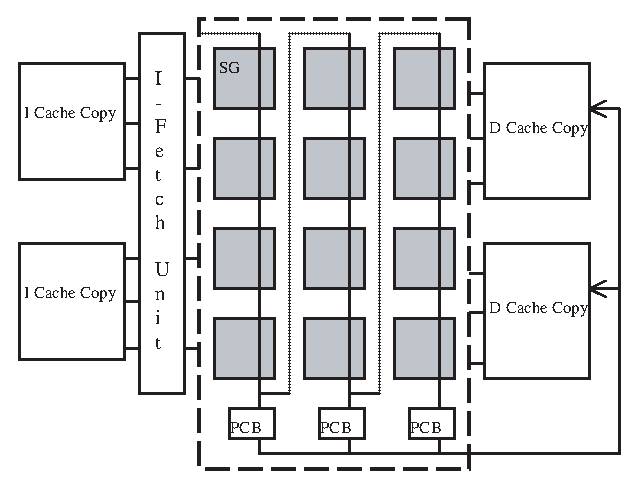
\epsfig{file=highlevel.eps,width=3.0in}
\caption{{\em High level diagram of our microarchitecture.}
Shown is the execution window, within the dashed box, along
with replicated instruction and data caches and the Previous
Column Buffers (PCB) at the bottom.}
\label{fig:highlevel}
\end{figure}
%
We are using a set of replicated
interleaved I-caches to satisfy our high fetch bandwidth requirements.
The instruction fetch unit loads instructions into the active
stations.  The key here is that instructions with small branch domain size
are normally fetched in the static or memory order.  This will simplify
the aligning and collapsing logic in the I-fetch unit and allows for
higher instruction fetch rates.
The major components of this microarchitecture are now discussed.

Figure~\ref{fig:execwind} shows a partial diagram of our execution
window with its subcomponents.   The execution window is the part
of Figure \ref{fig:highlevel} that was within the dashed rectangle.
%
\begin{figure}
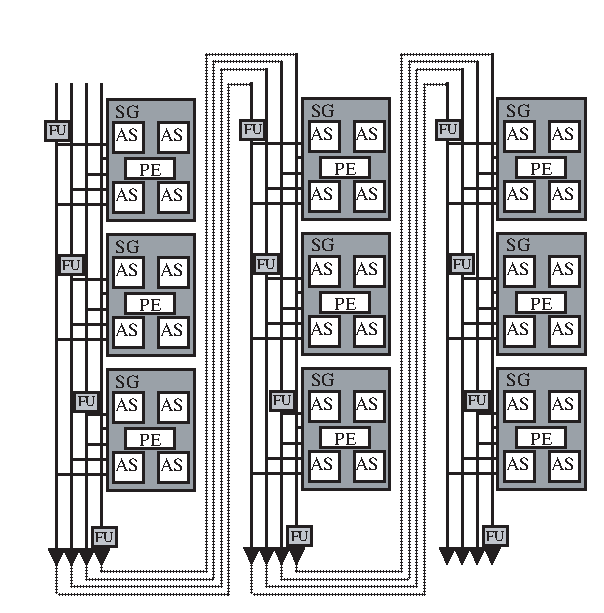
\epsfig{file=execwind.eps,width=3.0in}
\caption{{\em Interconnection fabric in the Execution Window.}
Sharing groups (SG) are shown interconnected with operand
transaction buses.  Sharing groups consist of a set of active
stations (AS) allong with processing elements (PE).
The buses are electrically repeated through the action of
forwarding units (FU).}
\label{fig:execwind}
\end{figure}
%
The active stations are laid out in a
two-dimensional grid.  Subsequent blocks of instructions are loaded
into each column and their transactions are forwarded down the column
and to the top of the next column.  
Active stations account for
most of the distributed control logic necessary for our
microarchitecture.  They correctly acquire instruction operands and 
enforce control and data dependencies
without
the need for any prior setup or data dependency initialization.  
The distributed
nature of active stations and their relatively localized interconnections
also helps to ensure a fast cycle time.

Dispersed among the active stations are associated \emph{processing elements}
(PE).  Processing elements may consist of an unified all-purpose
execution unit capable of executing any of the possible machine
instructions or, more likely, consist of several functionally
partitioned units individually tailored for specific classes of
instructions (integer ALU, FP or other), as is typical of most current
machines.

Groups of active stations along with their associated
processing elements are termed a sharing group (SG).
Similar to roles that the issue window, register file, executions units,
and the reorder buffer fulfill in
a conventional microarchitecture, sharing groups
have a relatively high degree of bus interconnectivity
within them.  The active stations
serve the role of both the reservation station and the reorder buffer
of more conventional machines.  
The transfer (issuing) of a decoded instruction,
along with its associated operands, from an AS to its PE are isolated to
within the given SG.  The use of this execution resource-sharing
arrangement also allows for reduced interconnections between adjacent
sharing groups.  Only operand results (including predicate operands)
need to flow from one SG to subsequent ones.
%
%
\subsection {Segmented Buses}
\label{sec:segbus}
%
An interconnection fabric is provided to forward result operands from
earlier active stations to later active stations in dynamic program order.  
The
interconnect allows for an arbitrary number of sharing groups to be used
in a machine while still keeping all bus spans to a constant length.
All the buses in Figure~\ref{fig:execwind} form the interconnection
fabric.  The width of the buses can be increased by using several buses
in parallel, which increases the overall available bus bandwidth.

Active bus repeater components are required to allow for constant
length bus spans.  Adjacent bus segments are connected 
with \emph{F{il}ter Unit} (FU) components.  
These units do more than just repeat operand values from one
span of a bus to the next.  For registers and memory, operands are
f{il}tered so that redundant forwards of the same value are eliminated.
This f{il}tering provides a means to reduce the overall bandwidth
requirements of the forwarding interconnection fabric.
The f{il}tering is accomplished by retaining a copy of previously
forwarded operands.  If a new operand arrives to be forwarded,
its value is checked against what was forwarded previously.
Only operands with changed values that then forwarded.
This serves to better use the bus bandwidth on the next bus
segment by eliminating useless forwards.  Accordingly, bus bandwidth
in the whole of the execution window is saved.

There are three type of f{il}ter units, one according to each of the
operands types that are forwarded: register, memory, and predicate.
The \emph{Register F{il}ter Unit} (RFU), \emph{Memory F{il}ter
Unit} (MFU), and \emph{Predicate F{il}ter Unit} (PFU), each handle
one of the three types of operands respectively.
Each of these forwarding units also handles its
associated transactions for the type of operand it serves.
All f{il}ter units need to snoop the forwarding buses and snarf
values that have a time-tag greater or equal to the latest
snarfed value but which value is less than that of its own assigned
time-tag.  This is the same associated snooping requirement
for the active stations.
This ensures that the f{il}ter units always keep
the latest value for any register or memory operand address.

In the case of the RFU, each holds the most recent value
for each of the architected machine registers.  
This property is part of what allows for the complete elimination
of any centralized register f{il}e.
The
register values are forwarded to subsequent RFUs during the course of
program execution and therefore no single RFU always holds the
persistent architected register state, but rather this function rotates
among the RFUs that are in the execution window of the machine.
The RFUs could have also used register caches but then an alternative
means of maintaining persistent register state would be needed.
Alternatives have been explored but are not generally as attractive
as having the full compliment of architected registers in each RFU.

The MFU has basically the same structure of an RFU but instead
it uses a small
cache (an L0 cache) to store the latest forwarded memory values.
The L0 cache proves to be an effective device in reducing the number of
requests to L1 D-cache.
Among our f{il}tering units, the PFU
is the simplest ; all they need to do is to keep track of the
latest CEPB branch and forward it to the next bus span.
%
\begin{figure}
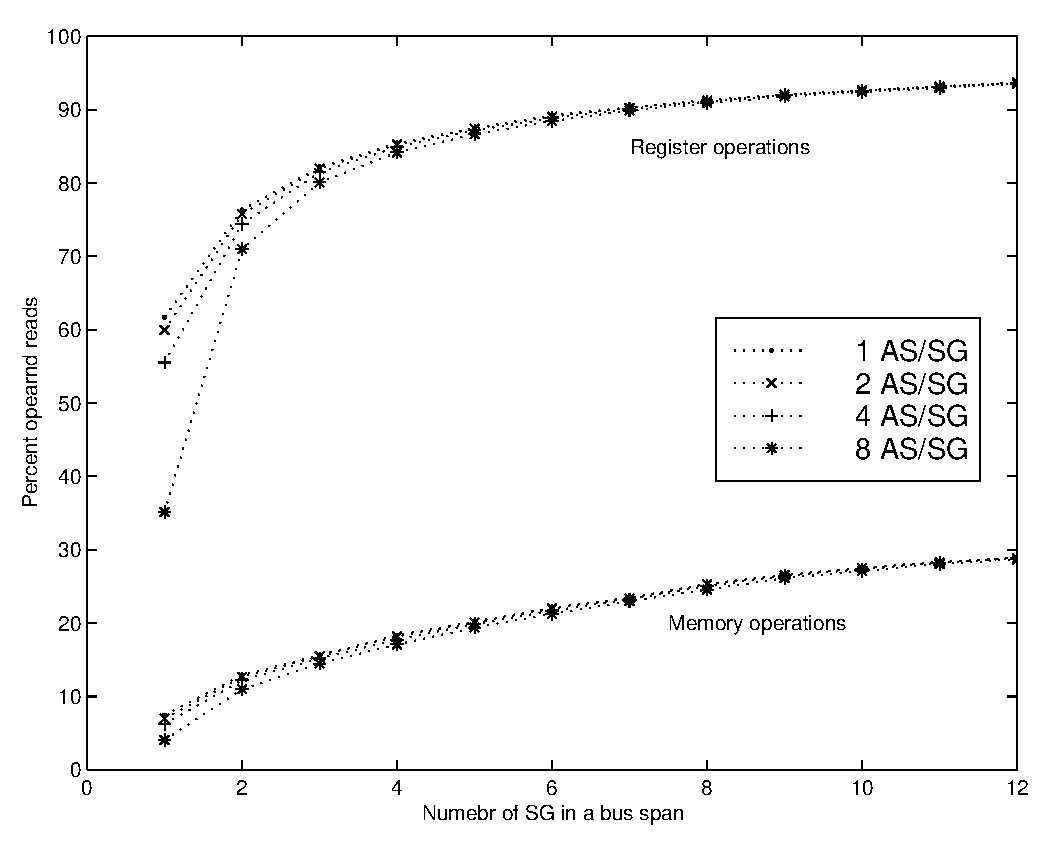
\epsfig{file=thrbussp.eps,width=3.0in}
\caption{{\em Read operations satisfied in single bus span.}
The top set of curves gives the percent distribution for
register read requests while the bottom set provides the
percent distribution for memory read (load) requests.}
\label{fig:busspan}
\end{figure}
%
Using register f{il}ter units in the way that we have
results in the elimination of any centralized
register f{il}e and simplifies instruction commitment.  By the time
the instructions in a column have gone through their f{in}al execution
and the column is ready to retire, the RFU's in this column have
already forwarded the register values to the RFU's in the later
columns.  This eliminates the necessity of saving the ISA register
state in a separate register f{il}e.

As can be seen in Figure ~\ref{fig:execwind}, the buses extend from the
bottom of each column to the top of the next column.  
The bottom of the last column in the execution window is also 
connected to the top of the f{ir}st column.  It is important to note
that in the physical layout the distance between f{ir}st and last columns 
is not any greater than two adjacent columns.  This is due to the 
fact that columns create a loop where there is not really a
f{ir}st or last column but there are \emph{earliest loaded column} (ELC)
and the \emph{latest loaded column} (LLC).  The operand values are
forwarded from each column to the next column, except for the LLC
column which will forward its operand values only when a new column
is loaded with a new set of instructions.

The bus span length has a major effect on the
performance of this microarchitecture.
A short bus span means that many operand values
have to go through multiple f{il}ter units until they are
snooped by their dependent instructions.  On the other hand,
a large bus span might result in increased bus delay due to technology
implementation issues and can
translate into longer clock cycles as a result.  
Our goal is to keep the
cycle-time low while getting the most performance out of 
the microarchitecture.

To estimate the
effect of the bus span, we f{ir}st define the \emph{Def-Use distance}
metric for register and memory operations.

\textbf{Definition:}
Consider a pair of instructions $(I_i,I_j)$ in the dynamic
program order such that:
%
\begin{enumerate}
\item $I_i$ has the same output operand as one or more input operands of $I_j$.
\item There is no other instruction $I_k$ between $I_i$ and $I_j$ with the same
output operand as $I_i$.
\end{enumerate}
%
We define the Def-Use distance $DU(I_i,I_j)$ between instructions
$I_i$ and $I_j$
as the number of instruction in the dynamic program order
between $I_i$ and $I_j$, including $I_j$ itself.
We also define $P_{du}(d)$ as the probability that an instruction
has a Def-Use distance of $d$.
Using the above definitions, we will estimate the
fraction of all the instructions that have a Def-Use distance
less than or equal to a given bus span.

We can assume that each instruction has an
equal probability of being assigned to any active station.  
Let $n$ be
the number of active stations within a register bus span 
length and $m$ be the
number of active stations per sharing group.  
Referring to Figure~\ref{fig:execwind},
we can see that all reads from instruction $I_j$ in the last 
active station $AS_j$,
for which $DU(I_i,I_j) < n$ will be satisfied through an 
instruction $I-i$ in the
same bus span.  
Similarly, all reads from instruction $I_{j-1}$ for which
$DU(I_i,I_{j-1})<n-1$ will be also satisfied on the same bus span.  
Extending this argument to all the instructions in a sharing group, 
we can show that
the ratio of all read operations that can be satisfied by 
a write operation in the same bus span is:

\[
\frac{1}{m}\left[\sum_{i=1}^{n-1} P_{du}(i) + 
\sum_{i=1}^{n-2} P_{du}(i) + \cdots +
\sum_{i=1}^{n-m} P_{du}(i)\right]
\]

This same formula can be applied for both register and memory operations by
using their corresponding $P_{du}$ probability.

To develop an estimate for the def-use probability $P_{du}$, we 
ran a set of programs from the SpecInt-2000 and SpecInt-95 benchmark
suites and measured the def-use distance for each operand
in the program execution.

%To develop an estimate for the def-use probability $P_{du}$, we ran 
%the set of programs 
%in table~\ref{tab:benchmark} and measured Def-Use distance for each operand
%address. The benchmarks in table~\ref{tab:benchmark} consist of seven
%programs form the SpecInt-2000 suite and three form the SpecInt-95 suite.
%All programs were compiled using the SGI compiler on the
%SGI IRIX 6.4 operating system.
%Programs were compiled with standard optimization (-O) using
%(-mips1) switch. The f{ir}st 600 million instruction of all programs
%were executed and data was only collected after the execution of the
%f{ir}st 100 million instructions.

%
%\begin{table*}
%\begin{center}
%\caption{Benchmarks.}
%\label{tab:benchmark}
%\scriptsize{
%\begin{tabular}{|l|c|c|c|c|c|}
%\hline
%Benchmark&Load&Store&Cond.&Forw. Cnd.&Branch \\
%& & & Branch& Branch & Misprd. \\
%\hline
%    bzip2   & 32\%  & 10\%  & 6\%   & 5\%   & 91.01\% \\
%    compress& 18\%  & 10\%  & 11\%  & 8\%   & 84.58\% \\
%    crafty  & 23\%  & 18\%  & 8\%   & 7\%   & 87.17\% \\
%    gcc & 23\%  & 15\%  & 15\%  & 11\%  & 92.03\% \\
%    go  & 21\%  & 9\%   & 12\%  & 10\%  & 80.8\% \\
%    gzip    & 21\%  & 8\%   & 8\%   & 6\%   & 84.28\% \\
%    ijpeg   & 18\%  & 8\%   & 6\%   & 4\%   & 86.41\% \\
%    mcf & 24\%  & 10\%  & 17\%  & 14\%  & 97.4\% \\
%    parser  & 28\%  & 9\%   & 11\%  & 9\%   & 90.58\% \\
%    vortex  & 29\%  & 20\%  & 9\%   & 7\%   & 98.43\% \\
%    Avg & 24\%  & 12\%  & 10\%  & 8\%   & 89.27\% \\
%\hline
%\end{tabular}
%}
%\end{center}
%\end{table*}
%

Figure ~\ref{fig:busspan} depicts the above formula for different values of
$m$ and $n/m$. the horizontal axis shows the bus span in terms of the number of
sharing groups in a bus span.  There are two sets of graphs in this figure,
one for register read operations and another for memory read operations.
Different lines in each set correspond to different values of
$m$ where \mbox{$m \in \{1,2,4,8\}$}.  
These graphs are especially interesting because they show that as the
bus span increases, the sensitivity to the number of active stations
per sharing groups is reduced.  A bus span of 8 captures more than 90\%
of register operation def-uses.  The fraction of captured memory
operations, however, is not very high.  This is due to the larger
memory def-use distances.

%\subsection{Early Notification}
%Limit the amount of speculation in order to reduce the bandwidth requirements.
%Based on the instruction type and operand address or history.
%
%
\subsection {Fetch and Dispatch}
%
The challenge in high bandwidth instruction fetch is mainly concerned
with the problem of multiple-branch prediction and aligning and
collapsing of multiple fetch groups.  One approach for solving this
problem has been focused on enhancing the instruction cache by using
multi-ported, multi banked copies of the instruction
cache~\cite{Yeh93b,Conte95,Seznec96,Wallace97}.
A more recent approach is the use of trace
caches~\cite{Rotenberg96,Jacobson97,Friendly97}.

To guide the fetch unit, a branch predictor capable of simultaneously
predicting multiple conditional
branches is used.  Examples of this sort of predictor can be found
in~\cite{Seznec96,Preston02}.  We are also
using a set of heuristics to guide I-fetch.  These heuristics are
developed to take advantage of the specific 
features of our microarchitecture
such as dynamic predication and multipath execution.
In the case of forward branches, we define two threshold values:
\emph{near} and \emph{far}.  We then compare the
branch domain size with the threshold values to categorize a
branch as one of \emph{near}, \emph{midway} or \emph{far}.

Since the domain of a forward branch with a near target
is small and can be easily
loaded within the execution window, the fetch unit will load the
instructions following the not-taken path of the branch, regardless of
its prediction.  This represents fetching of instructions in
the memory or static order rather than the program dynamic order and is
very common in the absence of a loop.  The fetching and loading of
instructions following the not-taken output path of a conditional
branch is advantageous for capturing hammock styled branch
constructs~\cite{Klauser98b}.  Simple single-sided hammock branches 
generally have
near targets and are captured within the execution window.  Our dynamic
predication scheme provides an efficient way for handling these kind of
branches using dynamic predication.

For a conditional branch with a moderate-distance target (neither
near nor far)
we use a confidence predictor
similar to the one described in ~\cite{Jacobsen96} to measure the
accuracy of the branch predictor.  If the branch is predicted with
high confidence, the instructions are fetched from the predicted
path.  Otherwise, fetch continues from
the sequential instructions after the branch.  By fetching the domain of
the branch, in case the branch is mispredicted, there is no need to flush the
execution window.  The dynamic predication scheme will change the input
predicates of the instructions within the domain of the branch (to become
enabled)
according to the outcome of the branch and
those instructions are re-executed as necessary.

In case of a conditional branch with a far target, 
we will always follow the predicted path to
avoid loading large number of useless instructions into the execution window.
The threshold values are parameters that can be either fixed at
design time or adaptively changed during the course of execution.  
We have only experimented with fixed threshold values in our research but
we are interested in evaluating other schemes.

If a conditional backward branch is predicted taken, it will be treated
as a loop and fetching and dispatch will follow the taken output path
of the branch.
This policy will basically unroll the loop and 
fill the whole of the execution window with
successive iterations of the loop.
These instructions will become one of multiple possible speculative
paths that can be accommodated simultaneously.
The instructions that constitute successive iterations of the
loop will become the \emph{main line} speculative execution path.
%
%Figure XXX shows an example of how this conversion is done.
%
A \emph{disjoint path} is also spawned to speculatively execute the
instructions following the not-taken outcome of the looping conditional
branch.
Note that multiple disjoint paths are possible from the not-taken
outcome of the conditional loop branch on each speculative loop iteration.
A more detailed discussion of multipath execution is discussed next.
%
%
\subsection{Multipath Execution}
%
Control-flow misprediction penalties pose an obstacle for
designing high performance microarchitectures.  Multipath
execution techniques have been proposed to reduce the effect of
mispredicted branches by executing instructions from both
outcome paths from a conditional branch ~\cite{Ahuja98}.

Uht showed ~\cite{Uht95} that both minimal control
dependencies and
\emph{Disjoint Eager Execution} (DEE) techniques are needed for 
extracting high IPC from sequential programs.
Disjoint Eager Execution gives 
execution priority to the instructions with the highest
likelihood of being committed.  In our microarchitecture, the
likelihood is not explicitly calculated; instead the \emph{static
tree} heuristic proposed by Uht ~\cite{Uht95} is used.  
This is a form of
multipath execution in which there is a predicted (main-line) path
as well as several much shorter not-predicted or \emph{disjoint}
paths spawned from the main-line path at some conditional
branches.

Disjoint paths are created by dispatching instructions to a free 
second column of 
active stations within a SG column.  Instructions from both main-line and
disjoint paths share the same PE and bussing resources in each
sharing group.  Active stations on the main-line path, however,
always have priority for the use of resources.  
In our present
microarchitecture, we always have two columns of active stations
within a SG, one for main-line path instructions and the other for disjoint
path instructions.
The f{ir}st AS column within each columns of SGs is reserved for the main-line
path of the program. 
The second column of active stations within each columns of SGs is
reserved for the possible execution of a disjoint path.  
Other arrangements are certainly possible but they have not yet been
explored.
To identify
the transactions associated with each disjoint path,
\emph{path\_ID's} are used.  
These are small integer numbers used to distinguish
between values generated by each path (whether it is the main-line path
or one of the disjoint paths).  
The main-line path has a path\_ID of zero.  
When a disjoint is spawned,
a transaction with the time-tag of the fork point $fork\_tt$ is forwarded.
Instructions on the disjoint path snoop for operand values and only snarf
those values from main-line path that have a time-tag less than $fork\_tt$.
The values with a time-tag greater than $fork\_tt$ are only snarfed if they
originated from the instruction on the same disjoint path.
The cost impact of realizing DEE is relatively low and is usually
less than 10\% increase in overall hardware for about a 45\% performance
improvement.

Main-line and disjoint paths execute concurrently, greatly reducing
branch misprediction penalties.  Conditional branches are assigned
to a free disjoint path (the path is \emph{spawned}) generally
assigned after they have been dispatched
into the execution window.  
The instructions comprising the disjoint path may be itself
dispatched to any column of ASes designated for that purpose (the
second AS column within each SG column).
This allows for multiple disjoint paths to be spawned from
conditional branches that may have all resided within a single
column of main-line path ASes.
At branch resolution,  if the disjoint path turns out to be the
correct path, it will replace the main-line path and the execution
will continue from there.
%
%
\subsection {Memory System}
%
Many studies show that incorporating techniques for reduction or
tolerance of memory latency, along with the design of high bandwidth memory 
interfaces are critical for achieving higher levels of IPC.  
Lockup-free caches~\cite{Kroft81}, prefetching~\cite{Chen94a,Fu92},
stream buffers~\cite{Palacharla94}, and
load prediction~\cite{lipasti96value} are among techniques that
have been proposed for reducing the frequency and impact of cache misses.  
High memory system bandwidth is typically achieved through 
interleaving and replication.

In this microarchitecture, the execution window offers another level of
caching for the memory values through the use of MFU's and
their associated L0 caches.  This extra caching also
reduces memory bandwidth requirements by satisfying
a fraction of loads from the previous stores in the execution window.
The store operations forward
their memory values that are snooped by both MFU's and load instructions.
The MFU's save the memory values in their L0 cache to be used for
servicing future backwarding requests from load instructions.

For those memory accesses that do not hit in an L0 cache, the requests
need to go to the higher levels of memory.  These requests 
are sent using a set of dedicated buses that connect each
sharing group to copies of the L1 data caches.  Since a load instruction
(dispatched to an AS) does not know
whether the memory value will bit in an L0 cache or need to be propagated to
an L1 cache, 
load requests are sent both on the backwarding bus (to possibly hit
in an L0 cache)
as well as directly to the L1 data cache through an additional bus.
This insures that no cycles
are wasted waiting for a response from an MFU for those cases 
that will be misses in all L0 caches that the load request might visit.
Other strategies are possible but this one has the general benefit of 
an overall low memory latency for satisfying load requests.

The next level of memory hierarchy is the L1-D cache.
To provide high memory bandwidth for our speculative microarchitecture,
L1 data caches are replicated, addresses
interleaved, and non-blocking.
All of these techniques provide for large access bandwidth
needed by our correspondingly larger execution window.

Committed writes to memory are handled through the
\emph{Previous Column Buffer} (PCB).
Upon commitment of the instructions in an SG column, 
the corresponding MFU's in that column are invalidated.  
This is necessary for limiting the maximum time-tag values
in our microarchitecture as well as suppressing unnecessary forwards of old
MFU values.  
The committed stores need to write their memory values to the
f{ir}st level data cache.  
During the course of execution, the PCB snoops
for all forwarded stores in the previous column and save the latest value
for each memory location (determined by address) seen.  
Multiple writes to the same
memory location are converted into a single write using the value
that occurs in later dynamic program order.
At commit time the PCB holds the latest memory values that need
to be
written to the L1 data cache.  This occurs through trough a set of 
interleaved buses.
Write updates are made to all copies of the L1 data cache at the same time.
The distributed organization of PCB's also helps to keep the cycle-time 
low since the stores do not to have 
to write to a single dedicated load-store buffer.
%
%
\subsection {Execution and Commitment}
%
Instructions that are fetched along one or more predicted paths are
decoded and staged into an instruction load
buffer and will be available to be dispatched into the execution
window.  Instructions are dispatched until all main-line AS columns
are full.
Every time the ELC column is retired,
a new set of instructions are dispatched to that AS column (making it
the new LLC).

Branch mispredictions can affect the execution in different
ways.  Speculative mispredictions of branches that have their domain
in the execution window results in a change of predicates and is 
handled through
the application of the resource flow dynamic predication scheme.
A conditional branch with a disjoint path that is
resolved as a mispredicted branch, will cause the disjoint path to
be switched to become the new main-line path.
If the branch is resolved to be not-taken, but was mispredicted and the
instructions following the branch target had been fetched into the window,
the execution window has to be \emph{flushed} and fetch
will resume following the not-taken outcome of the branch.

Active stations issue their instructions to the 
Processing Elements for execution.
In each sharing group, active stations with lower time-tag values are closer
to commitment and therefore have a higher priority for execution.
Among the main-line and disjoint path, main-line has higher priority
for using a processing element.

An AS column is retired when all of the instructions in the column have been
executed at least once and there are no more transactions on any 
interconnecting
buses between the sharing groups in the column.  This is locally
verified by each active station.  An active station such as $AS_i$
checks the status of the previous active station $AS_{i-1}$.  If
$AS_{i-1}$ is either committed or disabled and $AS_i$ does not have any
more transactions to send, then $AS_i$ is ready to commit.  The
commitment check is performed during the course of the execution and
does not impose any extra delay.  Instructions are gradually committed
from the top of the column while the instructions at the bottom of the
column might still be waiting for execution.
%
%
\section{Experimental methodology and results}
\label{sec:eval}
%
An execution driven simulator is written to model our
microarchitecture.  
The simulator supports the MIPS-1 ISA with some
MIPS-2 instructions also supported in order to accommodate code
residing in the SGI system libraries.  Table~\ref{tab:maconf} lists the
machine parameters that are used in our simulations. 
These values are representative of typical values 
for current microprocessors (2002).  
%
\begin{table}
\begin{center}
\caption{Default Machine Configuration}
\label{tab:maconf}
\scriptsize{
\begin{tabular}{|l|l|}
\hline
L0 cache size&32 words\\
\hline
L1 I/D cache access latency&1 clock\\
\hline
L1 I/D cache size&64 KBytes\\
\hline
L1 I/D block size&32 bytes\\
\hline
L1 I/D organization&2-way set assoc.\\
\hline
L2 cache access latency&10 clocks\\
\hline
L2 cache size&2 MBytes\\
\hline
L2 block size&32 bytes\\
\hline
L2 organization&direct mapped\\
\hline
main memory access latency&100 clocks\\
\hline
f{il}ter unit min. latency (all)&1 clock\\
\hline
forwarding-bus latency (all)&1 clock\\
\hline
number register buses&2\\
\hline
number predicate buses&1\\
\hline
number memory buses&2\\
\hline
branch predictor&PAg\\
\cline{2-2}
 & 1024 PBHT entries\\
\cline{2-2}
 & 4096 GPHT entries\\
\cline{2-2}
 & sat. 2-bit counter\\
\hline
\end{tabular}
}
\end{center}
\end{table}
%
We used ten benchmark programs from SpecInt-95 and SpecInt-2000
benchmark suites.  These programs were chosen to get a variety
of execution behavior.  All programs were compiled using the SGI vendor
compiler on the SGI IRIX 6.4 operating system using standard
optimization ({\tt -O}) and targeted for the MIPS-1 ISA ({\tt -mips1}).

A particular machine is generally characterized using the tuple:
%
\begin{itemize}
\item sharing group rows
\item active station rows per sharing group
\item sharing group columns
\end{itemize}
%
These three characteristic parameters of a given machine are
greatly influential to its performance, as expected, and is termed
the \emph{geometry} of the machine.  These three numbers are usually
concatenated.  For example the geometry of the machine in
Figure~\ref{fig:highlevel} would be abbreviated 3-4-3.

Figure~\ref{fig:geom} shows the IPC values for a range of machine sizes.
%
\begin{figure*}[bh]
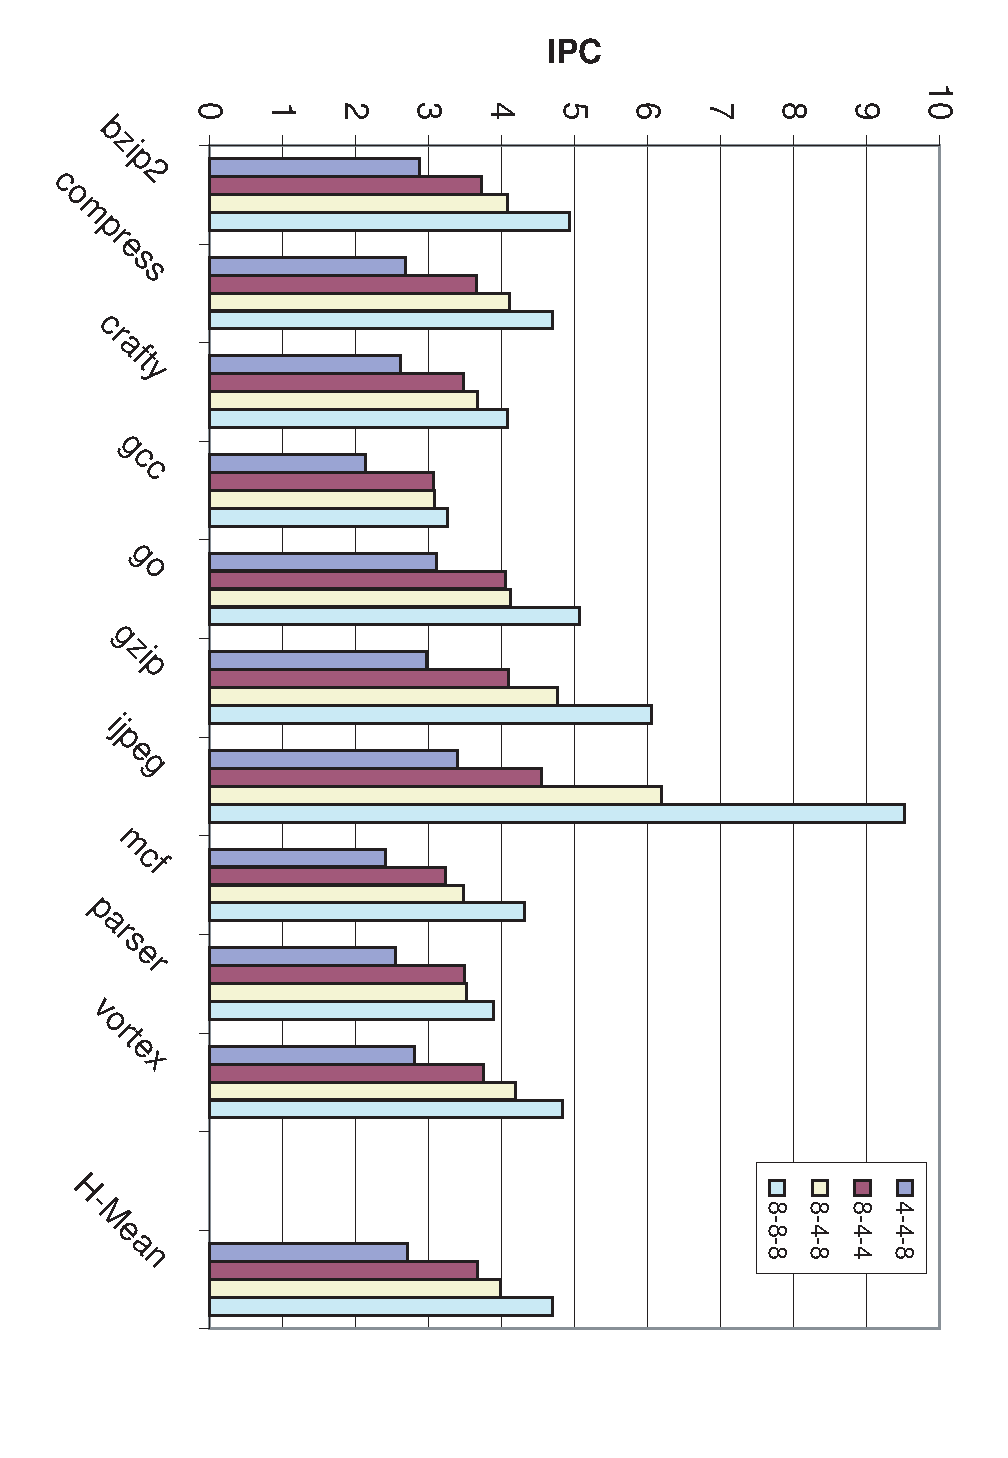
\epsfig{file=toc_geom.eps,angle=90,width=3.0in}
\caption{Effect of Geometry on IPC}
\label{fig:geom}
\end{figure*}
%
All machines simulated contained two forwarding buses for
register operands, two forwarding buses for memory operands, and
one forwarding bus for predicates.
Forwarding buses incur a bus transfer delay of 1 clock.
Further, each forwarding unit encountered 
has a minimum latency of 1 clock.
All simulated machines also have forwarding buses
that span eight Sharing Groups. 

%Machine sizes are characterized by three
%numbers that give the rows of SGs, the number
%of AS rows per SG, and the total number of 
%columns respectively.  The number of SG rows times the
%number of ASs per SG is the total number of
%AS rows in a configuration.  The product of all three
%numbers gives the total number of ASes in the machine and therefore
%the number of instructions that may be in flight 
%simultaneously

It can be seen that as the number of ASs increases,
the resulting IPCs also increase, but there are diminishing returns.
The main gain in IPC is achieved by going from 4-4-8 configuration 
to 8-4-8 configuration.  This is because the number of active stations
in each column is doubled and as a consequence, the fetch rate is also
doubled.  
Increasing the number of columns by going from 8-4-4 to 8-4-8 is less
beneficial.  This is due to the fact that in a configuration with more
columns, there is more chance for the instructions to be retired before
reaching the last column.  The number of columns, therefore, need to be
increased in proportion to the number of active station rows.

To get a better understanding of the potential speedup for this
microarchitecture, we simulated an 8-4-8 configuration with
some idealistic assumptions regarding fetch unit and memory
hierarchy.  Figure~\ref{fig:ideal} shows the simulation results.
The key to the configurations in this figure are as follows:
%
\begin{itemize}
\small{
\item IF: oracle branch predictor and infinite fetch bandwidth.
\item IM: infinite L1 cache size and infinite bandwidth.
\item RF: realistic fetch unit.
\item RM: realistic memory interface and limited cache size.
\item SP: single-path execution is assumed.
\item MP: static multi-path execution is assumed.
}
\end{itemize}
%
The IPC values from idealized cases put an upper limit on the amount of
parallelism that can be extracted from our microarchitecture.  From 
the graph in Figure ~\ref{fig:ideal} it is apparent that enhancing 
the fetch unit and reducing the branch misprediction penalties
should have the the greatest effect on the performance.  
%
\begin{figure*}[h]
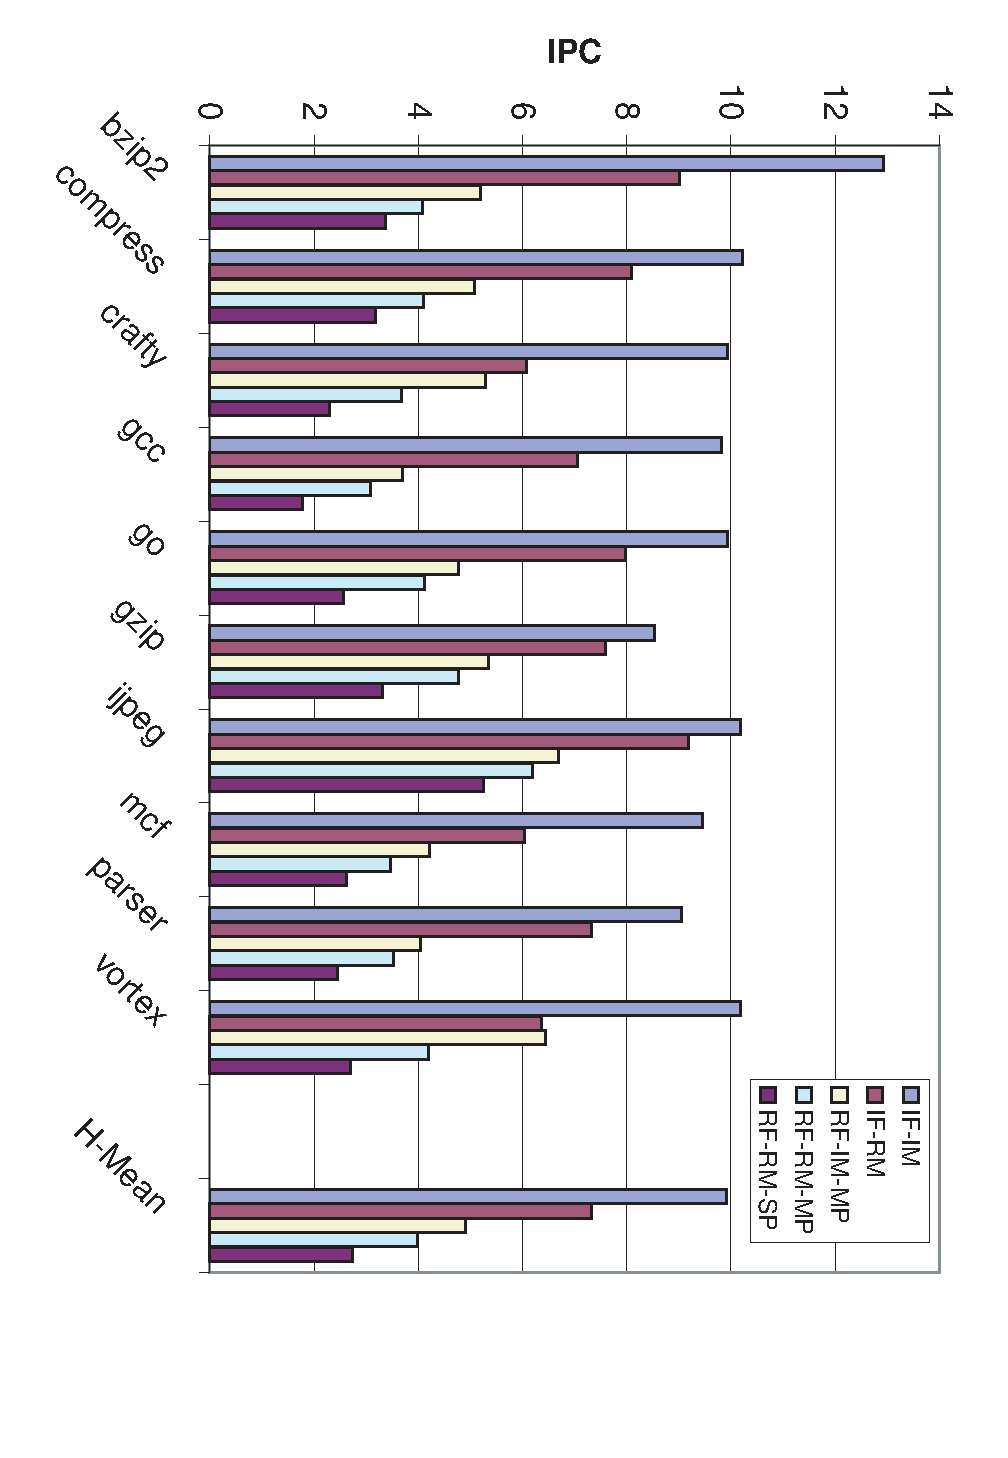
\epsfig{file=toc_ideal.eps,angle=90,width=3.0in}
\caption{Comparing ideal and realistic configurations.}
\label{fig:ideal}
\end{figure*}
%
Another important observation is that the IPC does not dramatically
drop when we use a realistic memory versus an ideal one.  The main 
reason is the use of L0 caches along with forwarding buses.  Our 
measurements show that, on average, in an 8-4-8 configuration, 34\% of
load operations are satisfied in the execution window, without having to
go to higher levels of memory.  This is achieved by either direct snooping
of forwarded memory values from previous memory store instructions
or through memory backward requests to the MFU's that
hit in an L0 cache.
%
%
%\subsection{Sensitivity Analysis}
%
%
\section{Conclusion}
%
In this paper we introduced the concept of Resource Flow execution
as a powerful approach for extracting higher levels of
parallelism through aggressive speculation.  Time-tags are used as a
method for tracking and enforcing program dependencies.  Novel
techniques for managing register, memory, and 
control-flow (predicate) dependencies were introduced.

Based on our Resource Flow execution model a new distributed
microarchitecture was proposed.  Physical scalability is achieved
through the use of a distributed microarchitectural components and a
segmented operand forwarding communication fabric.  Having no
centralized register file or reorder buffer relieves implementation
routing congestion that would affect large microarchitectures that
used those structures.
Access contention problems that cause operational
machine stalls is also largely eliminated.
The use of
time-tags allows for a degree of speculative execution that has not
been available in conventional microarchitectures.

Our initial simulations show encouraging IPC values with a potential
for extracting even higher IPC number from sequential code.  We are
currently pursuing improvements on I-fetch and multipath execution to
further enhance performance.

%
\bibliographystyle{latex8}
\bibliography{tocomputer}
%
\end{document}
%
%
